\documentclass[a4paper, toc=index, 12pt, DIV14, twoside, BCOR2cm, headsepline, numbers=noenddot, bibliography=totoc]{scrbook}

\usepackage{graphicx}
\usepackage{alltt}
\usepackage{url}
\usepackage{tabularx}
%\usepackage{ngerman}
\usepackage{longtable}
\usepackage[utf8]{inputenc}
\usepackage{tabularx}
\usepackage{listings}             % Include the listings-package
\usepackage{color}
\usepackage{graphicx}
\usepackage{caption}
\usepackage{subcaption}

\usepackage[T1]{fontenc}
\usepackage{ae, aecompl}
\usepackage{a4wide}
\usepackage{boxedminipage}
\usepackage{url}
\usepackage{graphicx}
\usepackage{enumerate}
\usepackage{float}
\usepackage{multicol}
\usepackage{tabularx}


\usepackage{ifthen}


\newenvironment{prettytablex}[1]{\vspace{0.3cm}\noindent\tabularx{\linewidth}{@{\hspace{\parindent}}#1@{}}}{\endtabularx\vspace{0.3cm}}
\newenvironment{prettytable}{\prettytablex{l X}}{\endprettytablex}
\setcounter{secnumdepth}{3}
\setcounter{tocdepth}{3}


\title{\huge\sffamily\bfseries System Description and Risk Analysis}
\author{Marc G\"ahwiler \and Leonhard Helminger \and Fabian Zeindler}
\date{21.11.2013}


\begin{document}
\maketitle

\tableofcontents
\pagebreak


\chapter{System Characterization}
\section{Introduction}
The company iMovies produces film material in the area of investigative journalism. To protect the integrity and the secrecy of email conversations within the company, a certificate based solution should be provided which ensures the confidentiality of these email conversations. \newline
The IT infrastructure of the company today divided into an internal network where the employees work with their desktop machines/laptops and a server area in which the a database server with user data, the web and email server as well as central storage for the employees is located. (this is an assumption by us, since there is no information about the status quo and iMovies is a relatively small company.) The status quo of the system is depicted in Figure \ref{oldsystem}.
\begin{figure}[H]
  \centering
    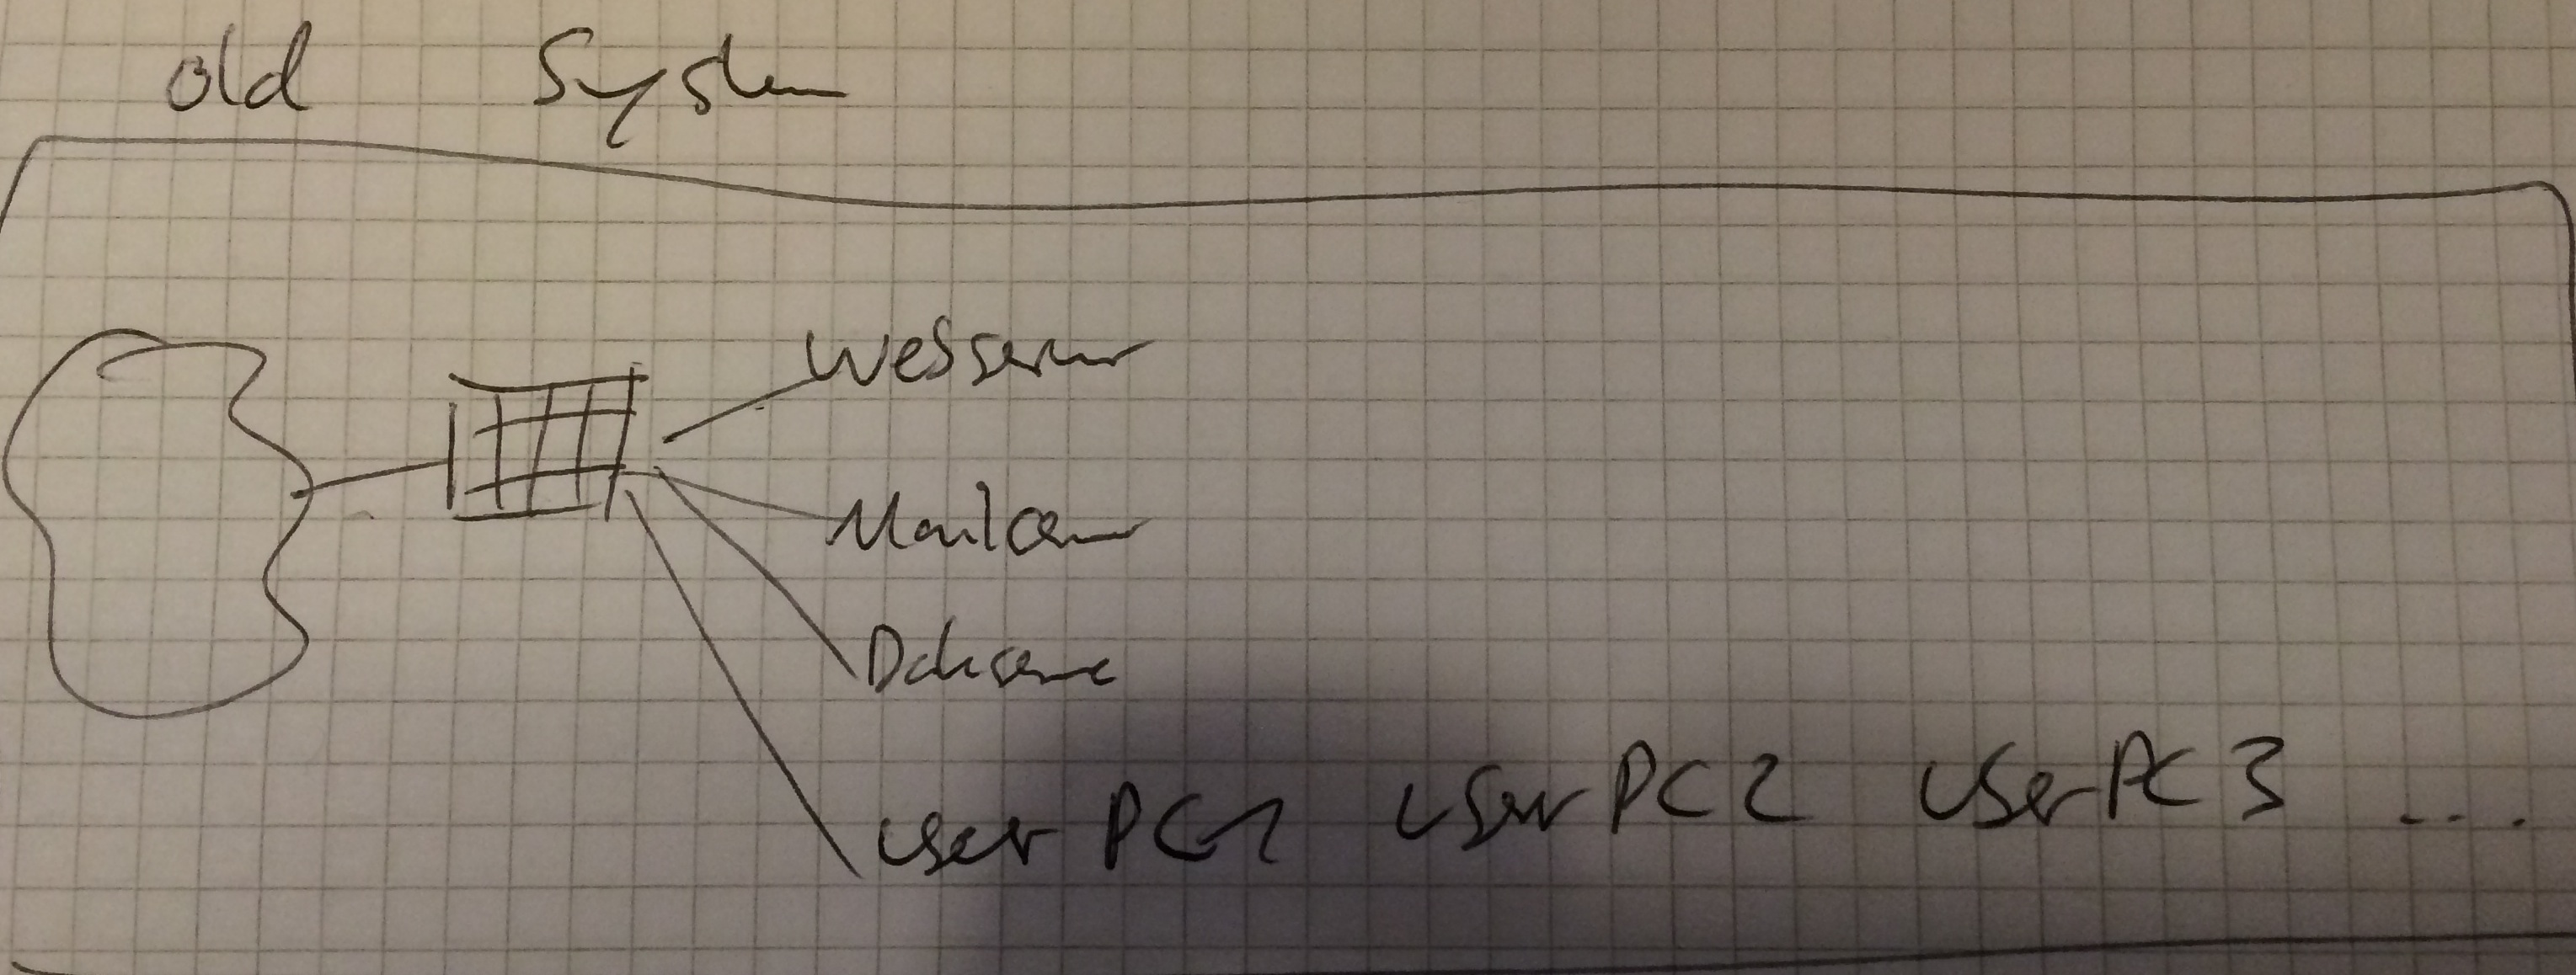
\includegraphics[width=0.6\textwidth]{images/oldsystem.jpg}  
  \caption{Diagram of the status quo.}
  \label{oldsystem}
\end{figure}

We now are challenged with the task to design and implement a certificate authority that provides the employees with digital certificates to be used to secure said email connections.\newline
This certificate authority should withstand targeted attacks and be integrated into the current system. For assigning employees to certificates, the already existing user database should be used. For securing the new build infrastructure, the old system also has to undergo some changes. We will introduce a new level of isolation for critical systems and put systems that do not have to be accessed directly by users in a separate part. The design of the system will be evaluated in detail in the following sections. An overview of the proposed system is shown in Figure \ref{newoverview}.
\begin{figure}[H]
  \centering
    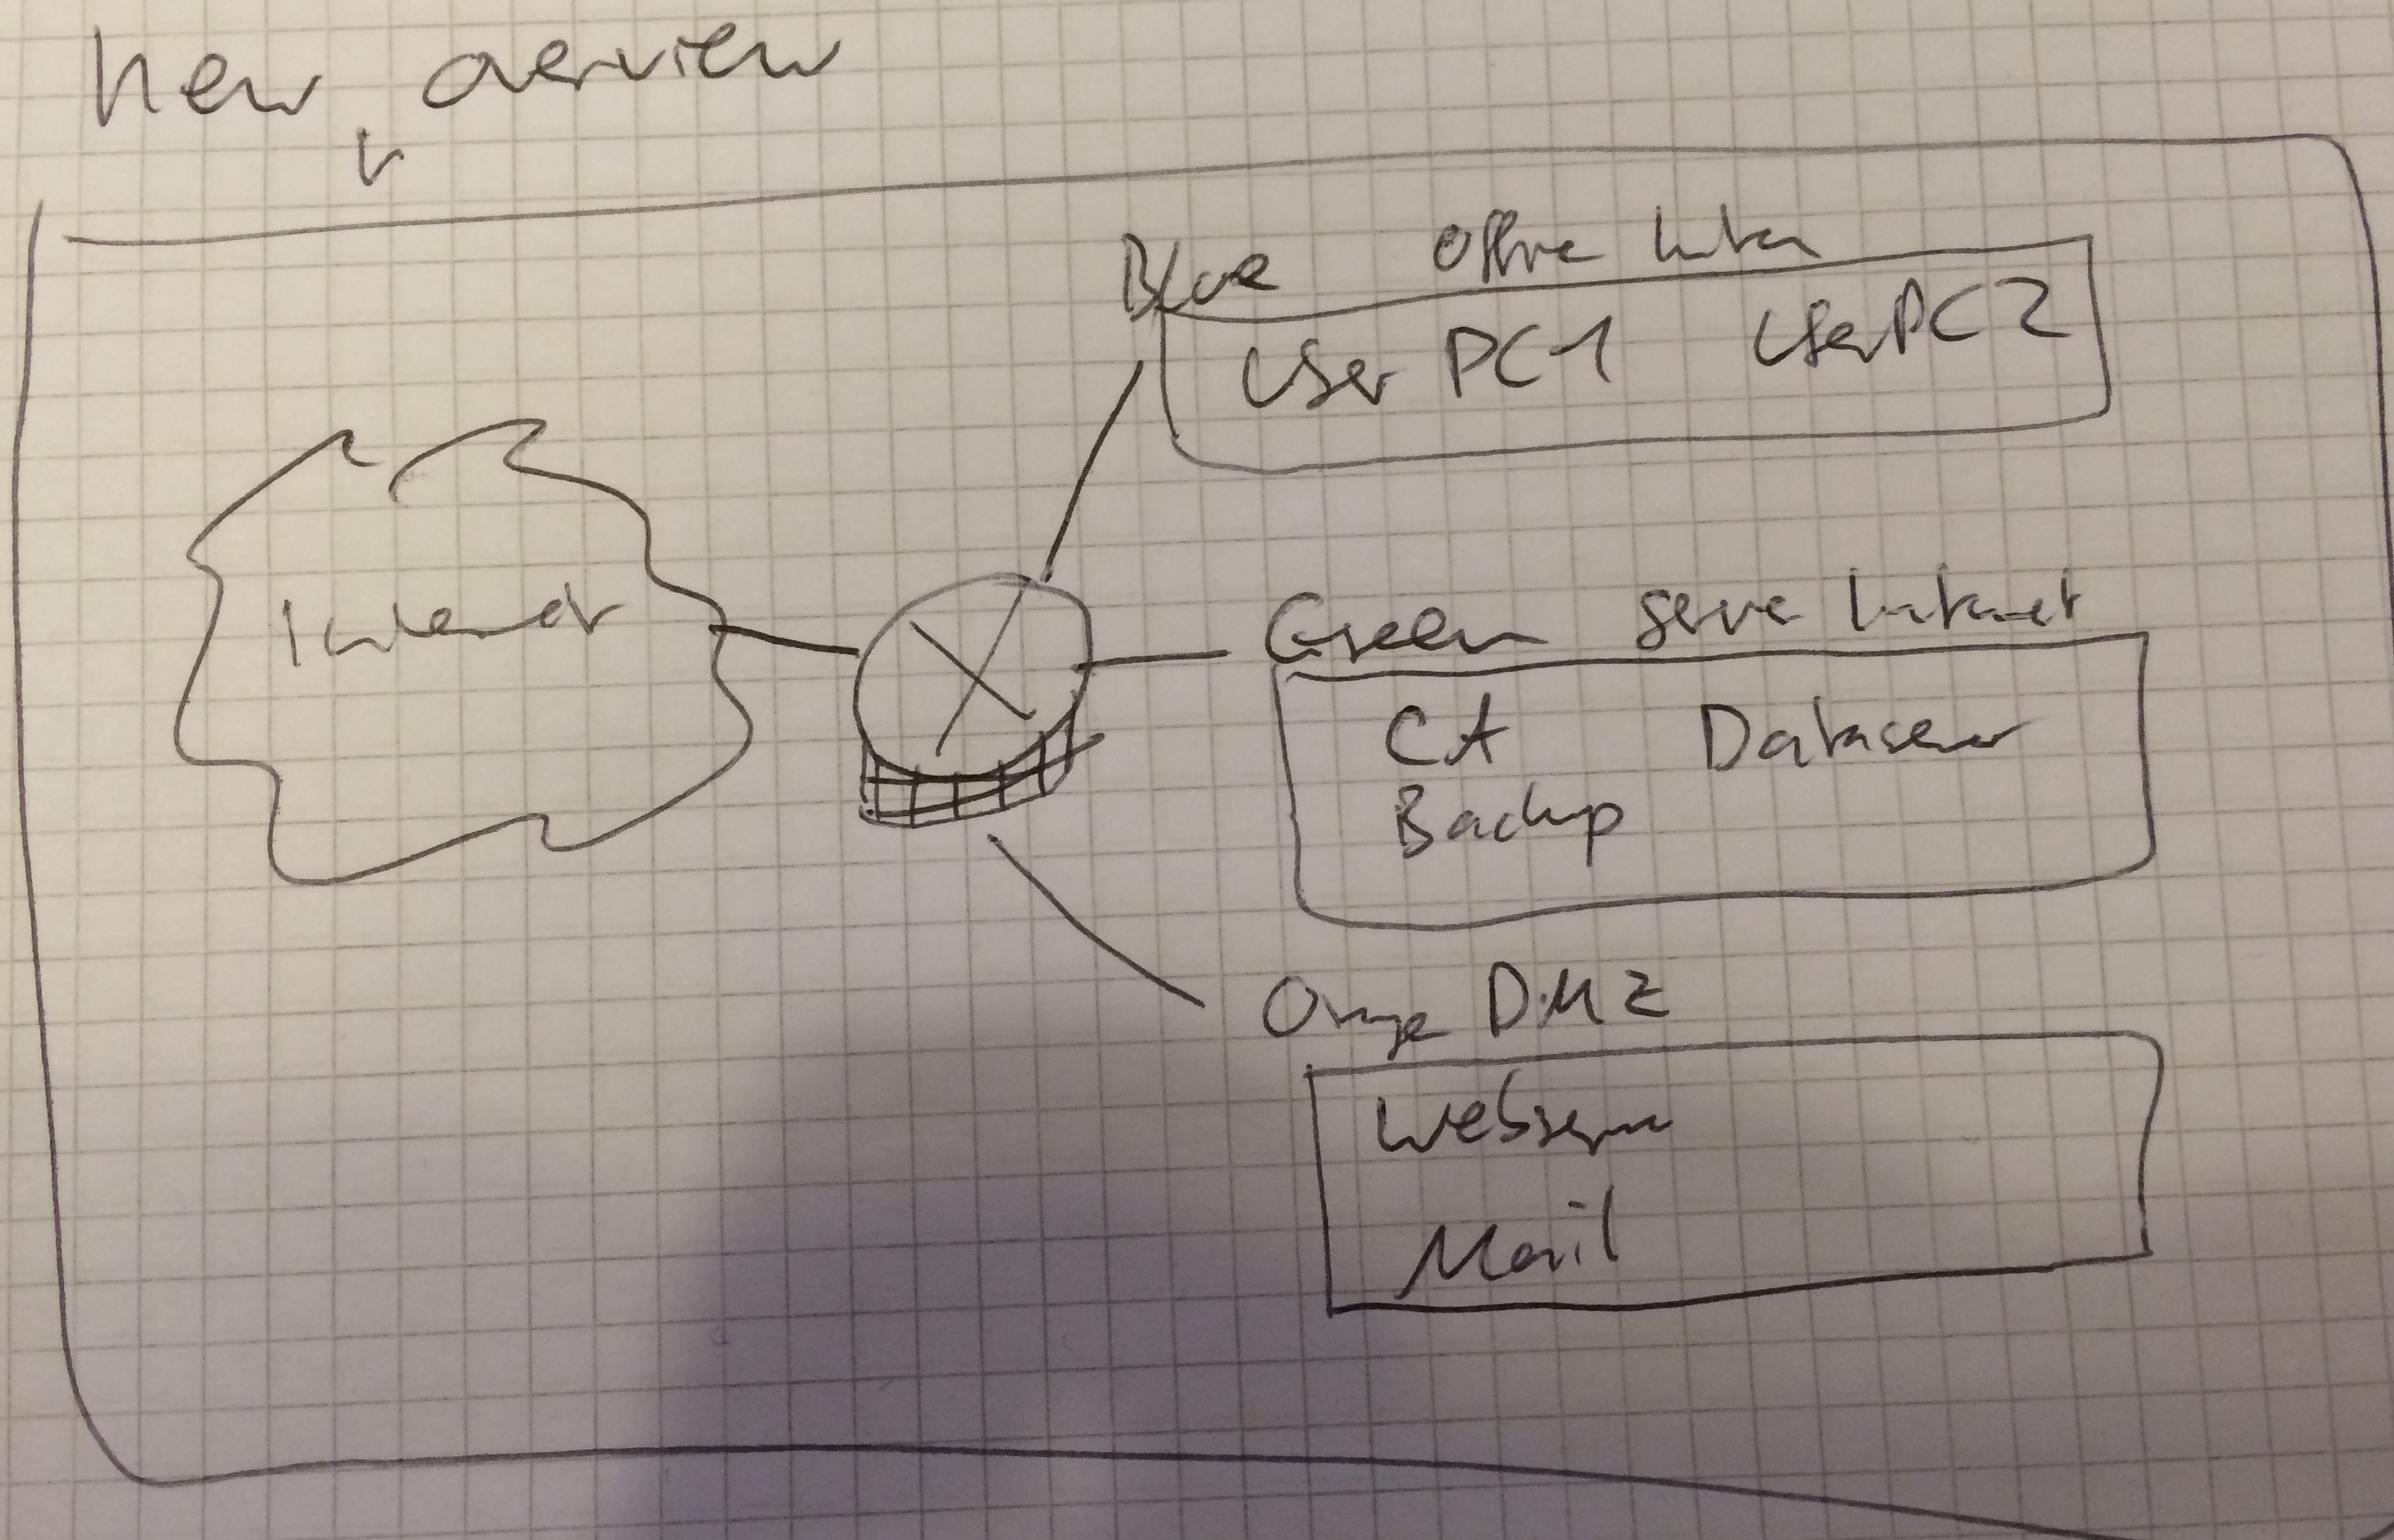
\includegraphics[width=0.6\textwidth]{images/newoverview.jpg}  
  \caption{Overview of the proposed system.}
  \label{newoverview}
\end{figure}

\section{System overview}
The employee will use the certificate authority such that he connects to a website with his credentials stored in the database. He then can issue a certificate or revoke existing certificates. When at least one certificate is obtained, login with said certificate is also possible. The user only has to deal with this web interface, but there is more to the system than that. A separate server is responsible for the process of actually issuing and revoking the certificates in compliance with the information stored in the database. This database could remain a separate instance, but for reasons of simplicity and since the company is small, we put the database on the same server as the CA core which implements the previously described functionality of issuing, verifying and revoking certificates. To prevent loss of data, ensure key recovery and auditability on the system in general, we implement a backup solution as well as a logging system and a key archive. These are all system that do not need regular and close interaction with users or even administrators. We therefore put them together on a backup and archive server, shielded from the outside.\newline
Since the user only interacts with the web interface which is publicly accessible, this is also the most exposed part of the system. We do not want it in close proximity of the most valuable part of the system, the core CA. We therefore set up a special demilitarized zone (DMZ) in which we place systems and functionality that has to be accessed from the outside. Every other functionality and system is not accessible from the outside and is placed in another zone.\newline
Figure \ref{systemoverview} shows the Webserver placed in the DMZ, the Core CA as well as the Backup/Archive server in an internal server zone. \newline
\begin{figure}[H]
  \centering
    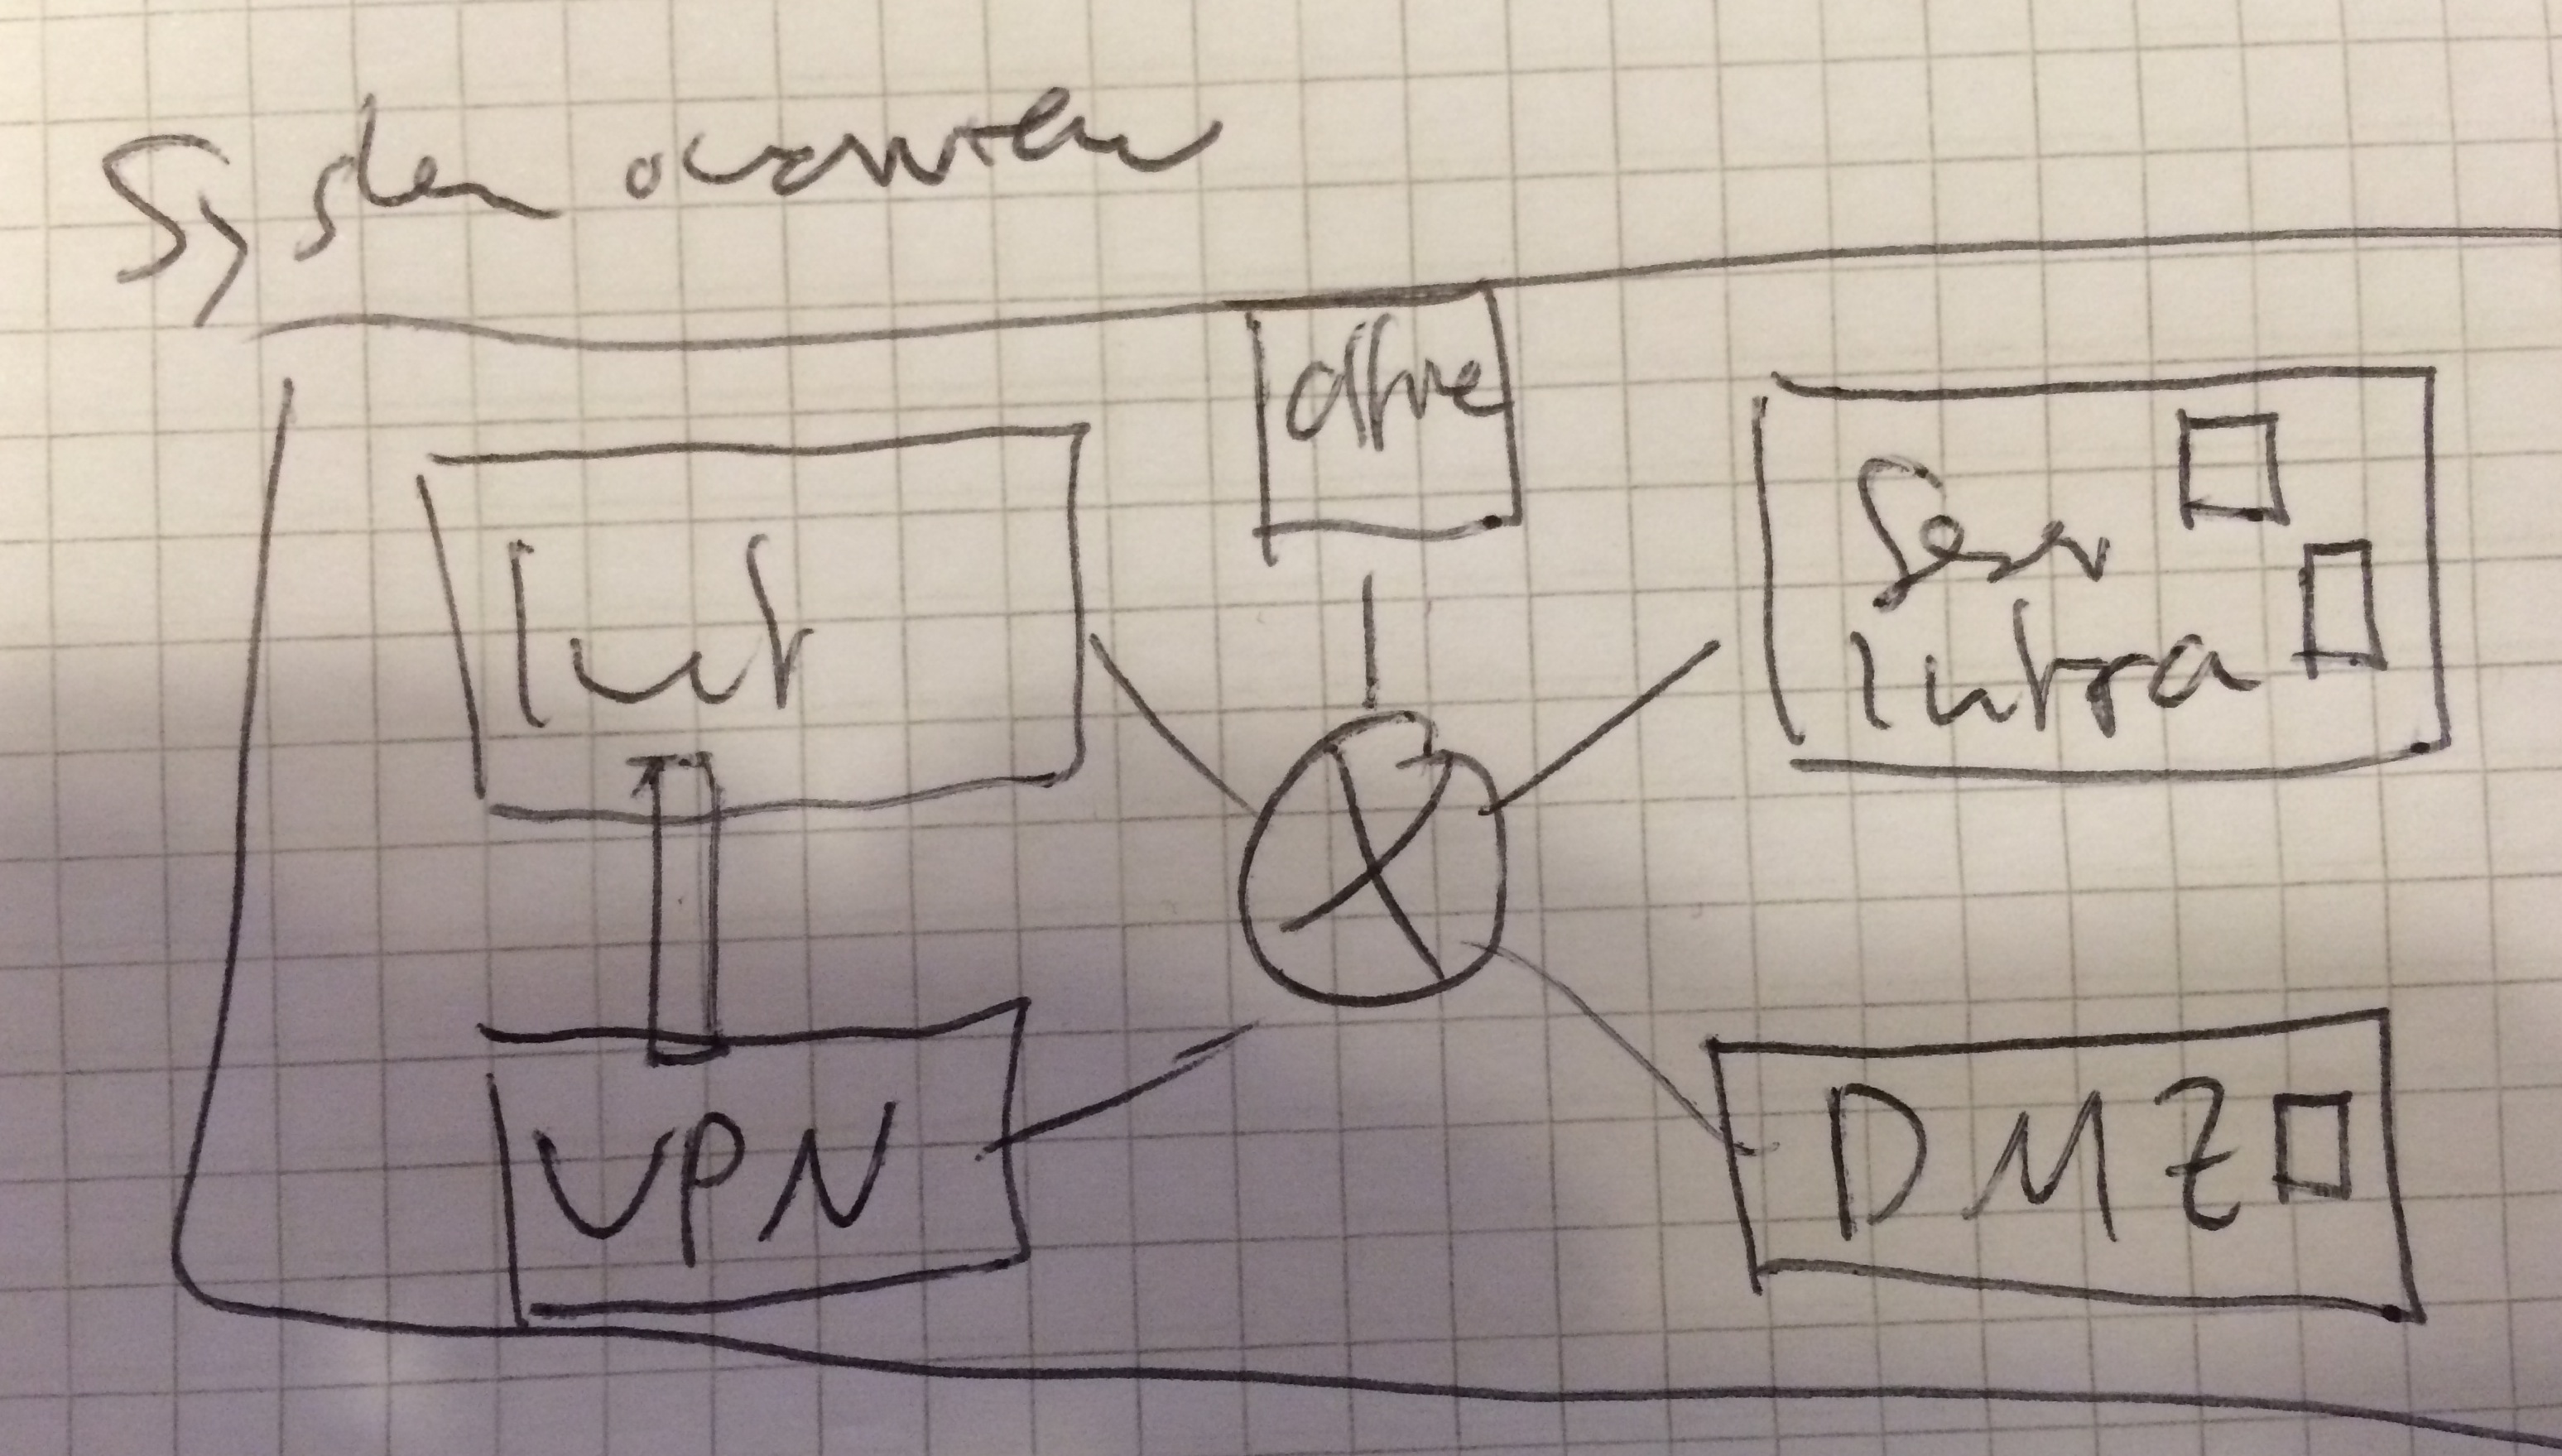
\includegraphics[width=0.6\textwidth]{images/systemoverview.jpg}  
  \caption{More detailed overview of the proposed system.}
  \label{systemoverview}
\end{figure}
The zone in which the employees have their personal machines in the office is also discrete from the zone with the Core CA, the database and the backup. It is shown in Figure \ref{systemoverview} but is not further discussed in this work, since the goal is to implement a certificate authority.\newline
For administrative remote access, we provide a VPN that allows an administrator to get access to all of these networks remotely.

We proceed with more detailed information about functionalities of the system and their implementation with special regard to security.

\section{Requirements elicitation and system functionality}
In this section we collect the requirements and the functionality of the proposed system. We first look at functional requirements to then give an insight in non functional requirements. We cover security requirements as a separate unit, since we want to emphasize the importance of these requirements to the certificate authority system.  
\subsection{Functional requirements}
We first list the functional requirements we extracted from the assignment we got to implement this system. From this these requirements we conclude general use cases of the system and will also give an insight in possible misuse cases.

\begin{description}

\item[User Interface: ]
A simple web interface which allows each user to log in either with his credentials from the legacy MySQL database, or one of his previously generated certificate and private key combinations.
Once logged in the user can view his information (last name, first name and email address), change his password and update his information (last name, first name and email address).
Additionally it is possible for the user to let the system issue a new certificate (based on his possibly changed credentials) and download the certificate with the newly generated private key in PKCS\#12 format.

\item[Administration Interface: ]
A simple web interface (not the same as the user web interface) where CA administrators can consult the current CA state after a log in process which requires the CA administrators to authenticate themselves with their certificate. This includes the number of issued certificates, the number of revoked certificates and the current serial number.

\item[Certificate Issuing and Revocation: ]
The CA offers an interface that allows other systems to
\begin{itemize}
\item Generate new public/private key pairs.
\item Generate a certificate that ties a public key to a user's credentials (first and last names and his email address) and sign this certificate with the CA's key.
\item Revoke a previously signed certificate.
\item Get a list that contains all revoked certificates (Certificate revocation list).
\end{itemize}

\item[Key Backup: ]
To prevent the loss of any information, that was encrypted with an issued certificate, every issued certificate and the according private key are archived.

\item[System Administration and Maintenance: ]
Each server is remotely accessible for the system administrator. Also the configuration of the systems running as well as the logging during operation is stored on the backup server.

\end{description}
\subsubsection{Use cases}
Figure \ref{usecase} shows the use cases in a graphical manner. We also list each use case individually with a short description.
\begin{figure}[H]
  \centering
    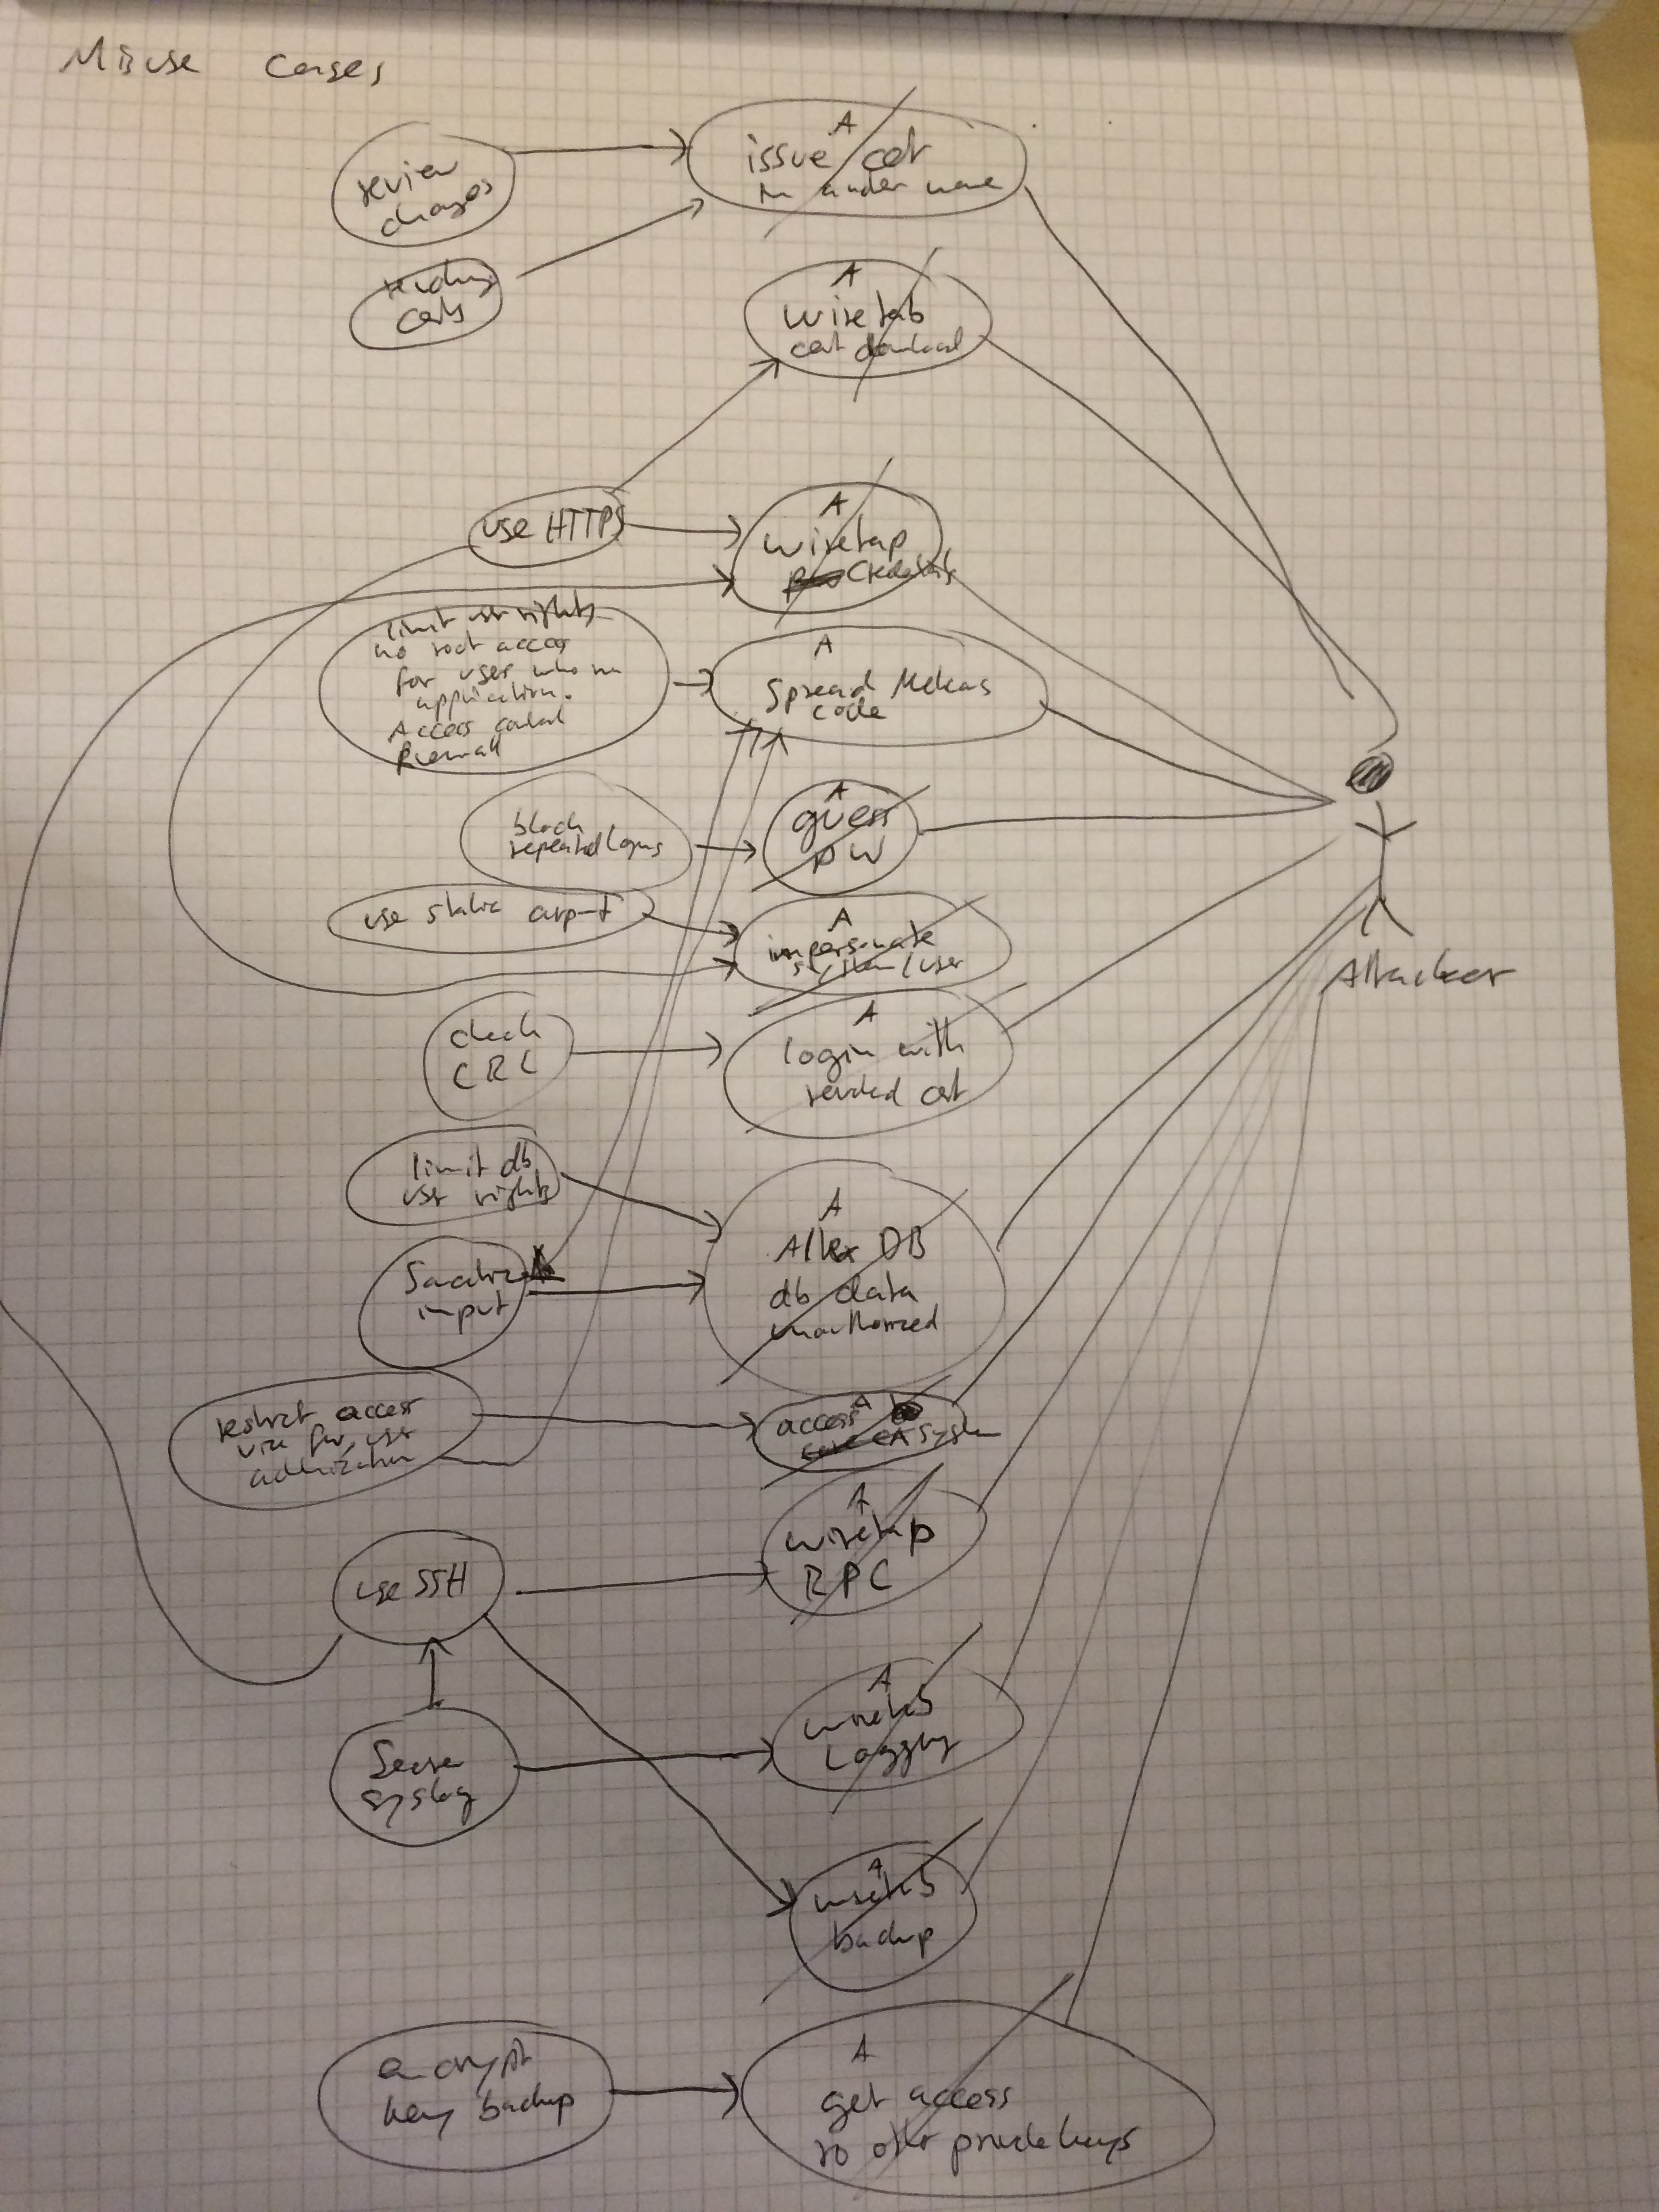
\includegraphics[width=0.6\textwidth]{images/usecase.jpg}  
  \caption{Use cases of the proposed system.}
  \label{usecase}
\end{figure}
We first identify the participating roles:
\begin{itemize}
\item User (The employee who uses the web interface to view/change user data, issue, verify, download, revoke certificates)
\item CA Administrator (Administrator who has access to certain CA information)
\item System Administrator (Administrator who can access all systems remotely)
\item Website/Webinterface (Displays information to users and CA Administrators)
\item Core CA (Issues, stores, revokes, verifies certificates)
\item Database (Stores user information)
\item Backup/Archive (Stores certificates, private keys, logging information, backed up configurations)
\end{itemize}
We now list the use cases of these roles:
\begin{description}
\item[Web login ] User logs onto the webserver with his credentials or a certificate.
\item[With certificate ] Login by presenting a certificate.
\item[With credentials ] Login by presenting user name and password.
\item[Verify credentials ] Presented credentials get verified against the information stored in the database (RPC call to CA Core).
\item[Validate certificate ] The presented certificate gets verified. CA Core ensures that it is a proper certificate and not yet revoked.
\item[Show user information ] The user information (except the password) stored in the database is displayed to the user (RPC call to the database).
\item[Change user data ] The user changes any of the information stored in the database.
\item[Review user data changes ] If a user changes information other than the password, the changes have to be reviewed by the CA Administrator before writing them to the database. All the users certificates get revoked.
\item[Request certificate ] A user sends a request for a new certificate (RPC call to CA Core).
\item[Issue certificate ] The CA Core issues a new certificate for the user who requested it. The certificate and the private key get archived.
\item[Download certificate ] The user can download its newly generated certificate and his private key.
\item[Backup keys ] After creating a new certificate, the CA Core also stores the new certificate and the according private key on the backup/archive server. 
\item[Revoke certificate ] A user or the CA Administrator set a certificate for revocation. (RPC call to CA Core).
\item[Generate CRL ] When revoking a certificate, the CA Core generates a new or updates an existing CRL.
\item[List CA information ] When a CA Administrator is logged in, his web interface displays the number of issued certificates, the number of revoked certificates and the current serial number.
\item[System login ] The System Administrator remotely logs into one of the running system and can get root access.
\item[Logging ] Each system automatically sends logging information of the system and the interactions with the system to the backup/archive server.
\item[Run backups ] The backup server periodically runs backups to collect the configurations of the other systems.
\item[Logout ] CA administrator and users that are logged in, can log out, which causes a new login prompt when visiting the site again.
\end{description}

\subsubsection{Misuse cases}
Figure \ref{misusecase} shows the misuse cases and also additional use cases that prevent this misuse cases in a graphical manner. We also list each misuse case individually with a short description.
\begin{figure}[H]
  \centering
    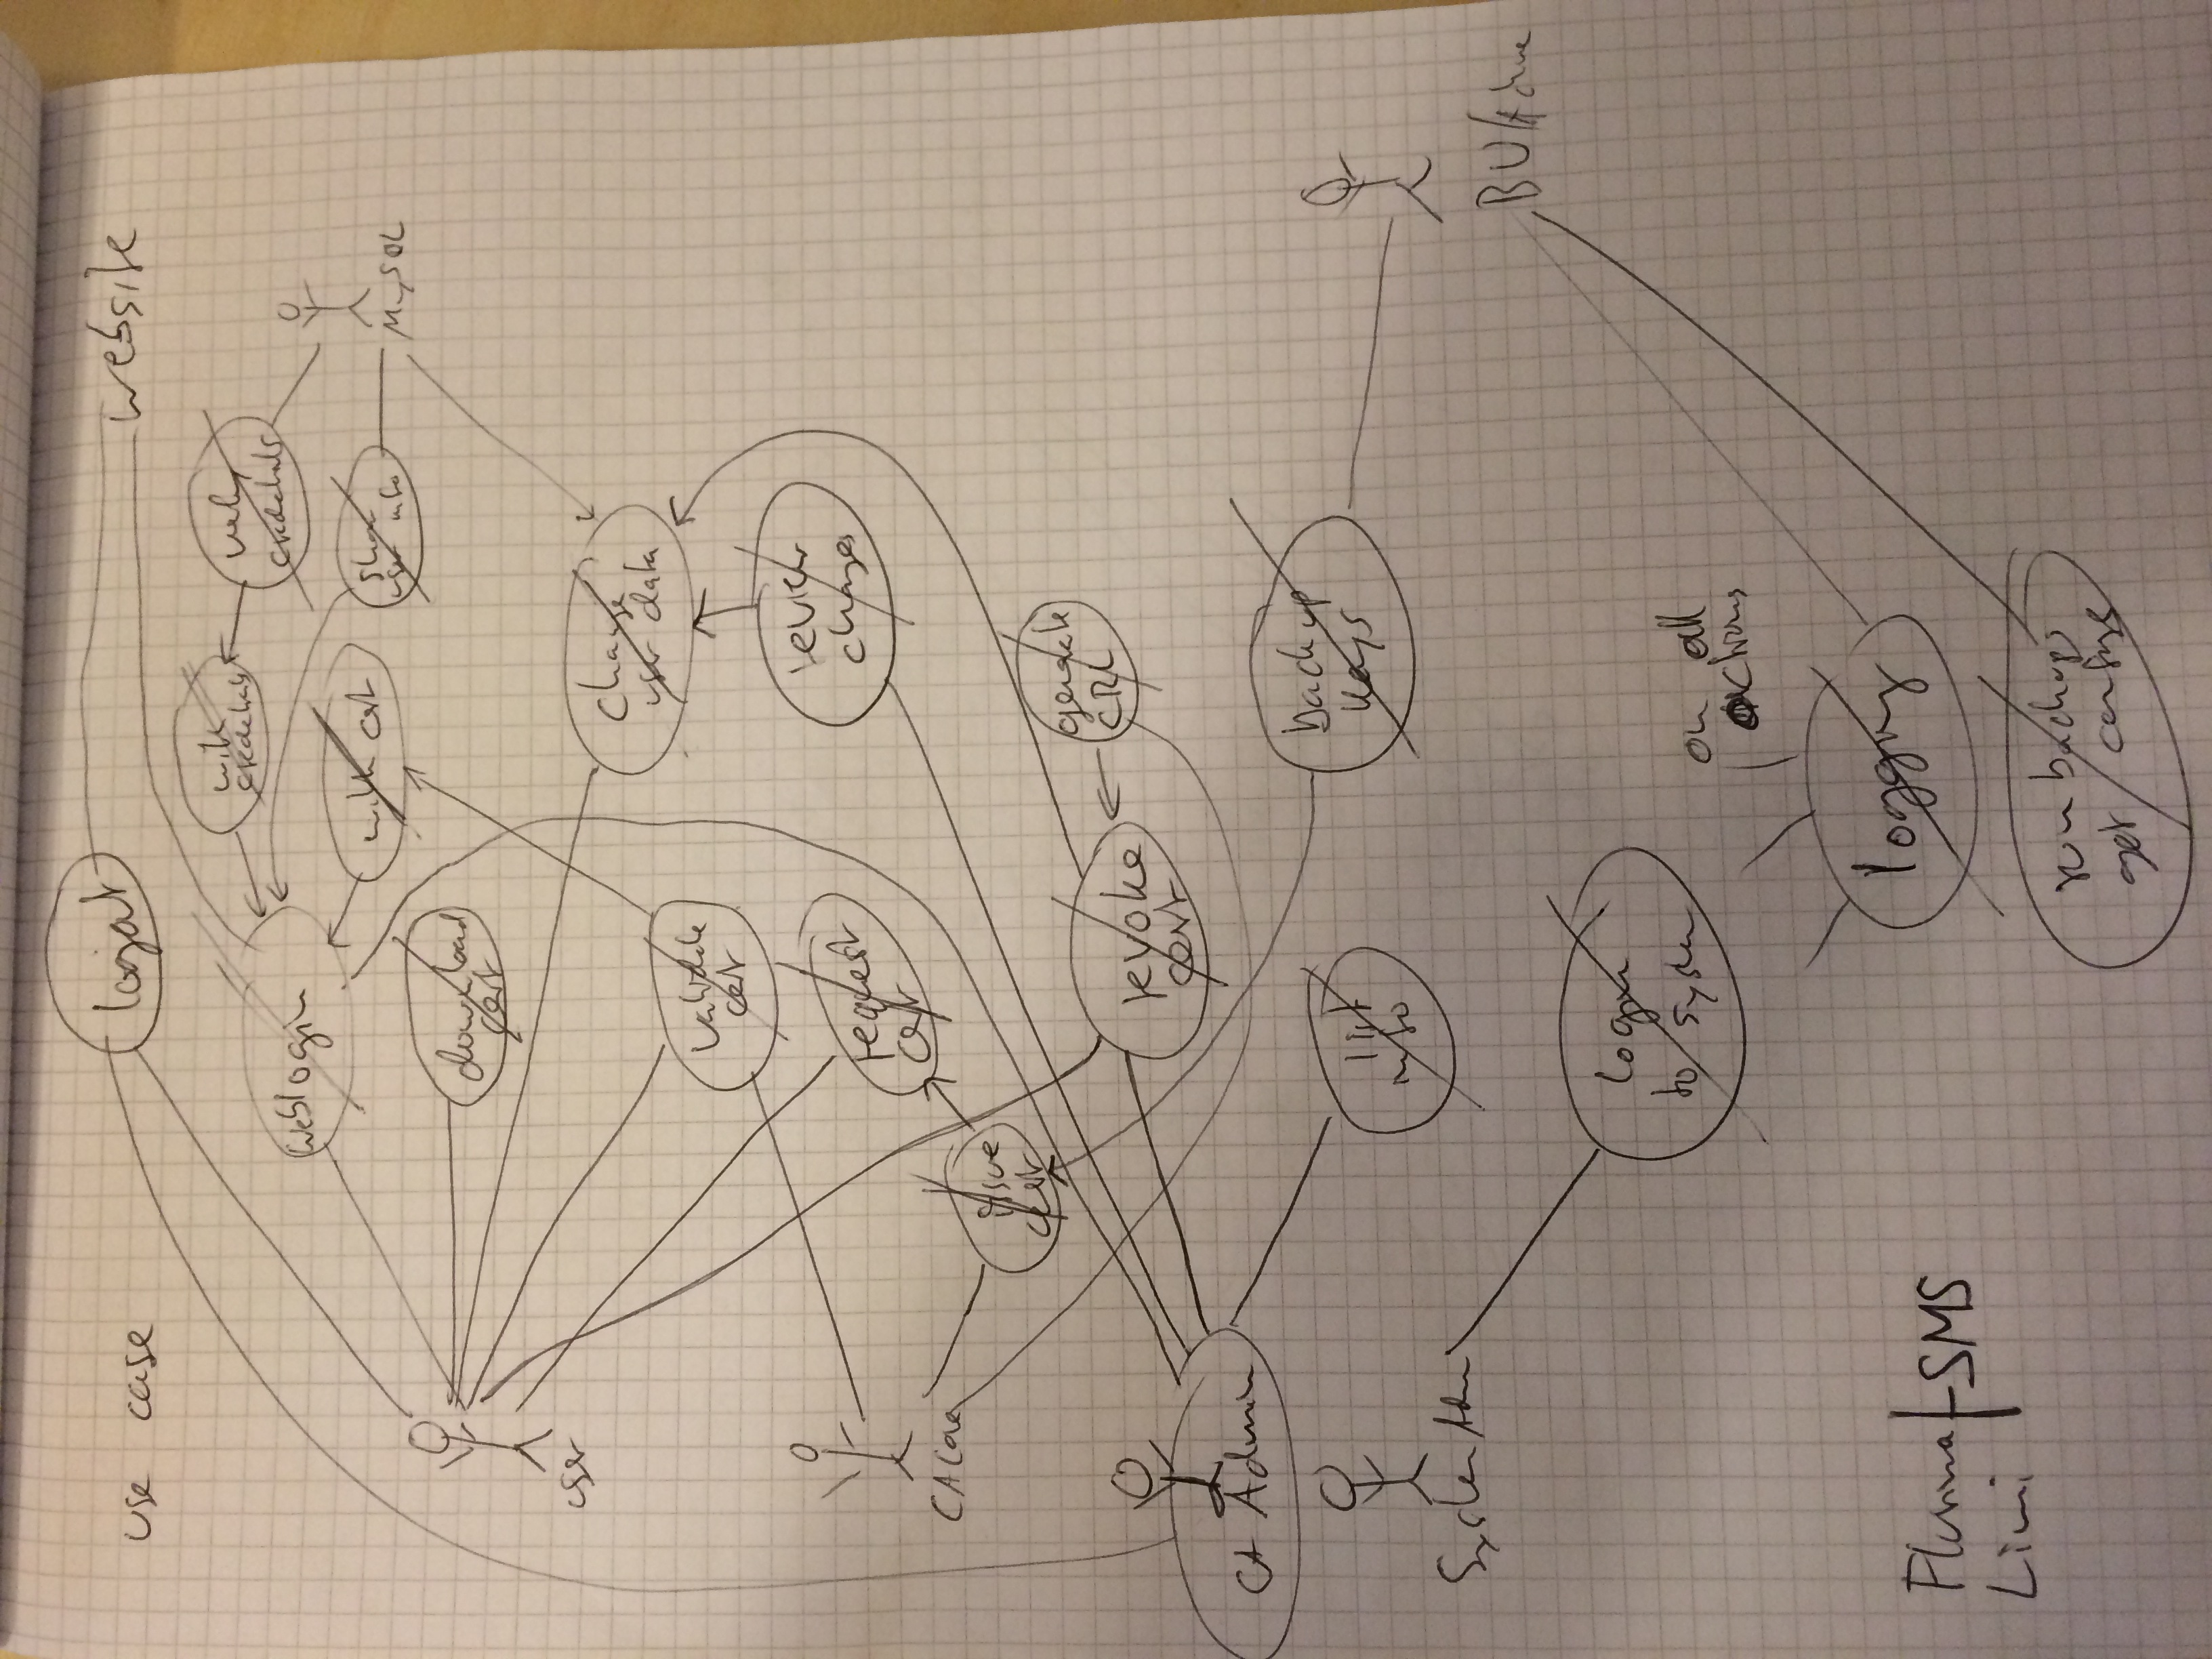
\includegraphics[width=0.6\textwidth]{images/misusecase.jpg}  
  \caption{Misuse cases and additional use cases of the proposed system.}
  \label{misusecase}
\end{figure}

We first identify the participating roles:
\begin{itemize}
\item Thread agent (The attacker which can be an outsider as well as an misbehaving employee)
\end{itemize}
We now list the misuse cases of these roles as well as the preventing use cases:
\begin{description}
\item[Issue certificate in another name ] The attacker is able to alter his information and then issue a certificate with this information. This gets prevented by the CA Administrator reviewing changes other than to the password and revoking all its issued certificates.
\item[Wiretap certificate download ] The attacker can obtain a copy of the certificate/private key pair of a user. This is prevented with enforcing HTTPS when connecting to the webservice.
\item[Wiretap user credentials ] The username and password get obtained by the attacker during transmission. This is prevented with enforcing HTTPS when connecting to the webservice. For system administrator credentials, use SSH and VPN to connect to remote systems.
\item[Guess password ] With multiple guesses, the attacker can bruteforce the password. To prevent this, limit the number of times a password for a given user can be tried.
\item[Impersonate system/user ] An attacker can spooth and poison communication mechanisms to impersonate a certain role. Use HTTPS and SSH to prevent this. In the infrastructure controlled by iMovies, use static ARP tables to prevent poisoning.
\item[Login with revoked certificate ] The attacker may get access to the system with presenting an invalid certificate. To prevent this, always check the CRL.
\item[Alter database date unauthorized ] An attacker alters data in the database that does not belong to him. To prevent this, one can sanitize the input, review all changes to the database by the CA Administrator and restrict the database user to only the functionality he needs.
\item[Access systems ] The attacker can login to the server systems. This is prevented by enforcing access control, only allowing certain traffic through the firewall and onto the system.
\item[Access other private keys ] The stored private keys in the archive get obtained by the attacker. To prevent this, the private keys are stored encrypted.
\item[Wiretap RPC ] An attacker obtains information transmitted between the webserver and the CA Core. To prevent this, the RPC traffic is tunneled via SSH.
\item[Wiretap logging ] The logging information from the servers and applications sent to the backup server gets obtained by the attacker. To prevent this, secure syslog is used which uses an SSH tunnel.
\item[Wiretap backup ] The attacker obtains system and configuration information by intercepting the backup transmission. SSH is used for backup to prevent this.
\item[Running malicious code ] An attacker is able to run malicious code on one of the systems. To prevent this, the users executing this systems have limited rights, strong access controls are implemented and input is sanitized.
\end{description}


\subsection{Non functional requirements}
The following list specifies non functional requirements gathered during the analysis.
\begin{itemize}
\item For the user database, the legacy database in MySQL has to be used.
\item New certificates and their private key are issued in the PKCS\#12 format.
\item Users with a valid certificate can authenticate them self over SSL/TLS to the website using the certificate. 
\item THERE IS MORE, BUT IT IS LATE...
\end{itemize}

\subsection{Security requirements}
Since the system is developed to bring more security to the way employees communicate, we honor the security requirements in a separate section. The following list is compiled from the initial assignment as well as from issues that arise from the misuse case diagram.
\begin{itemize}
\item Access control to CA Core functionality and data.
\item Secrecy and integrity of private keys in the archive.
\item Integrity, non-repudiation and accountability of log files on the backup server.
\item Secrecy and integrity of the user data stored in the database.
\item Access control on all systems.
\item Confidentiality, integrity and authenticity with regards to key transport.
\item Secrecy and integrity of CA Core data during processing and transport.
\item THERE IS MORE, BUT IT IS LATE...
\end{itemize}

\section{Components and Subsystems}
\begin{figure}[H]
  \centering
    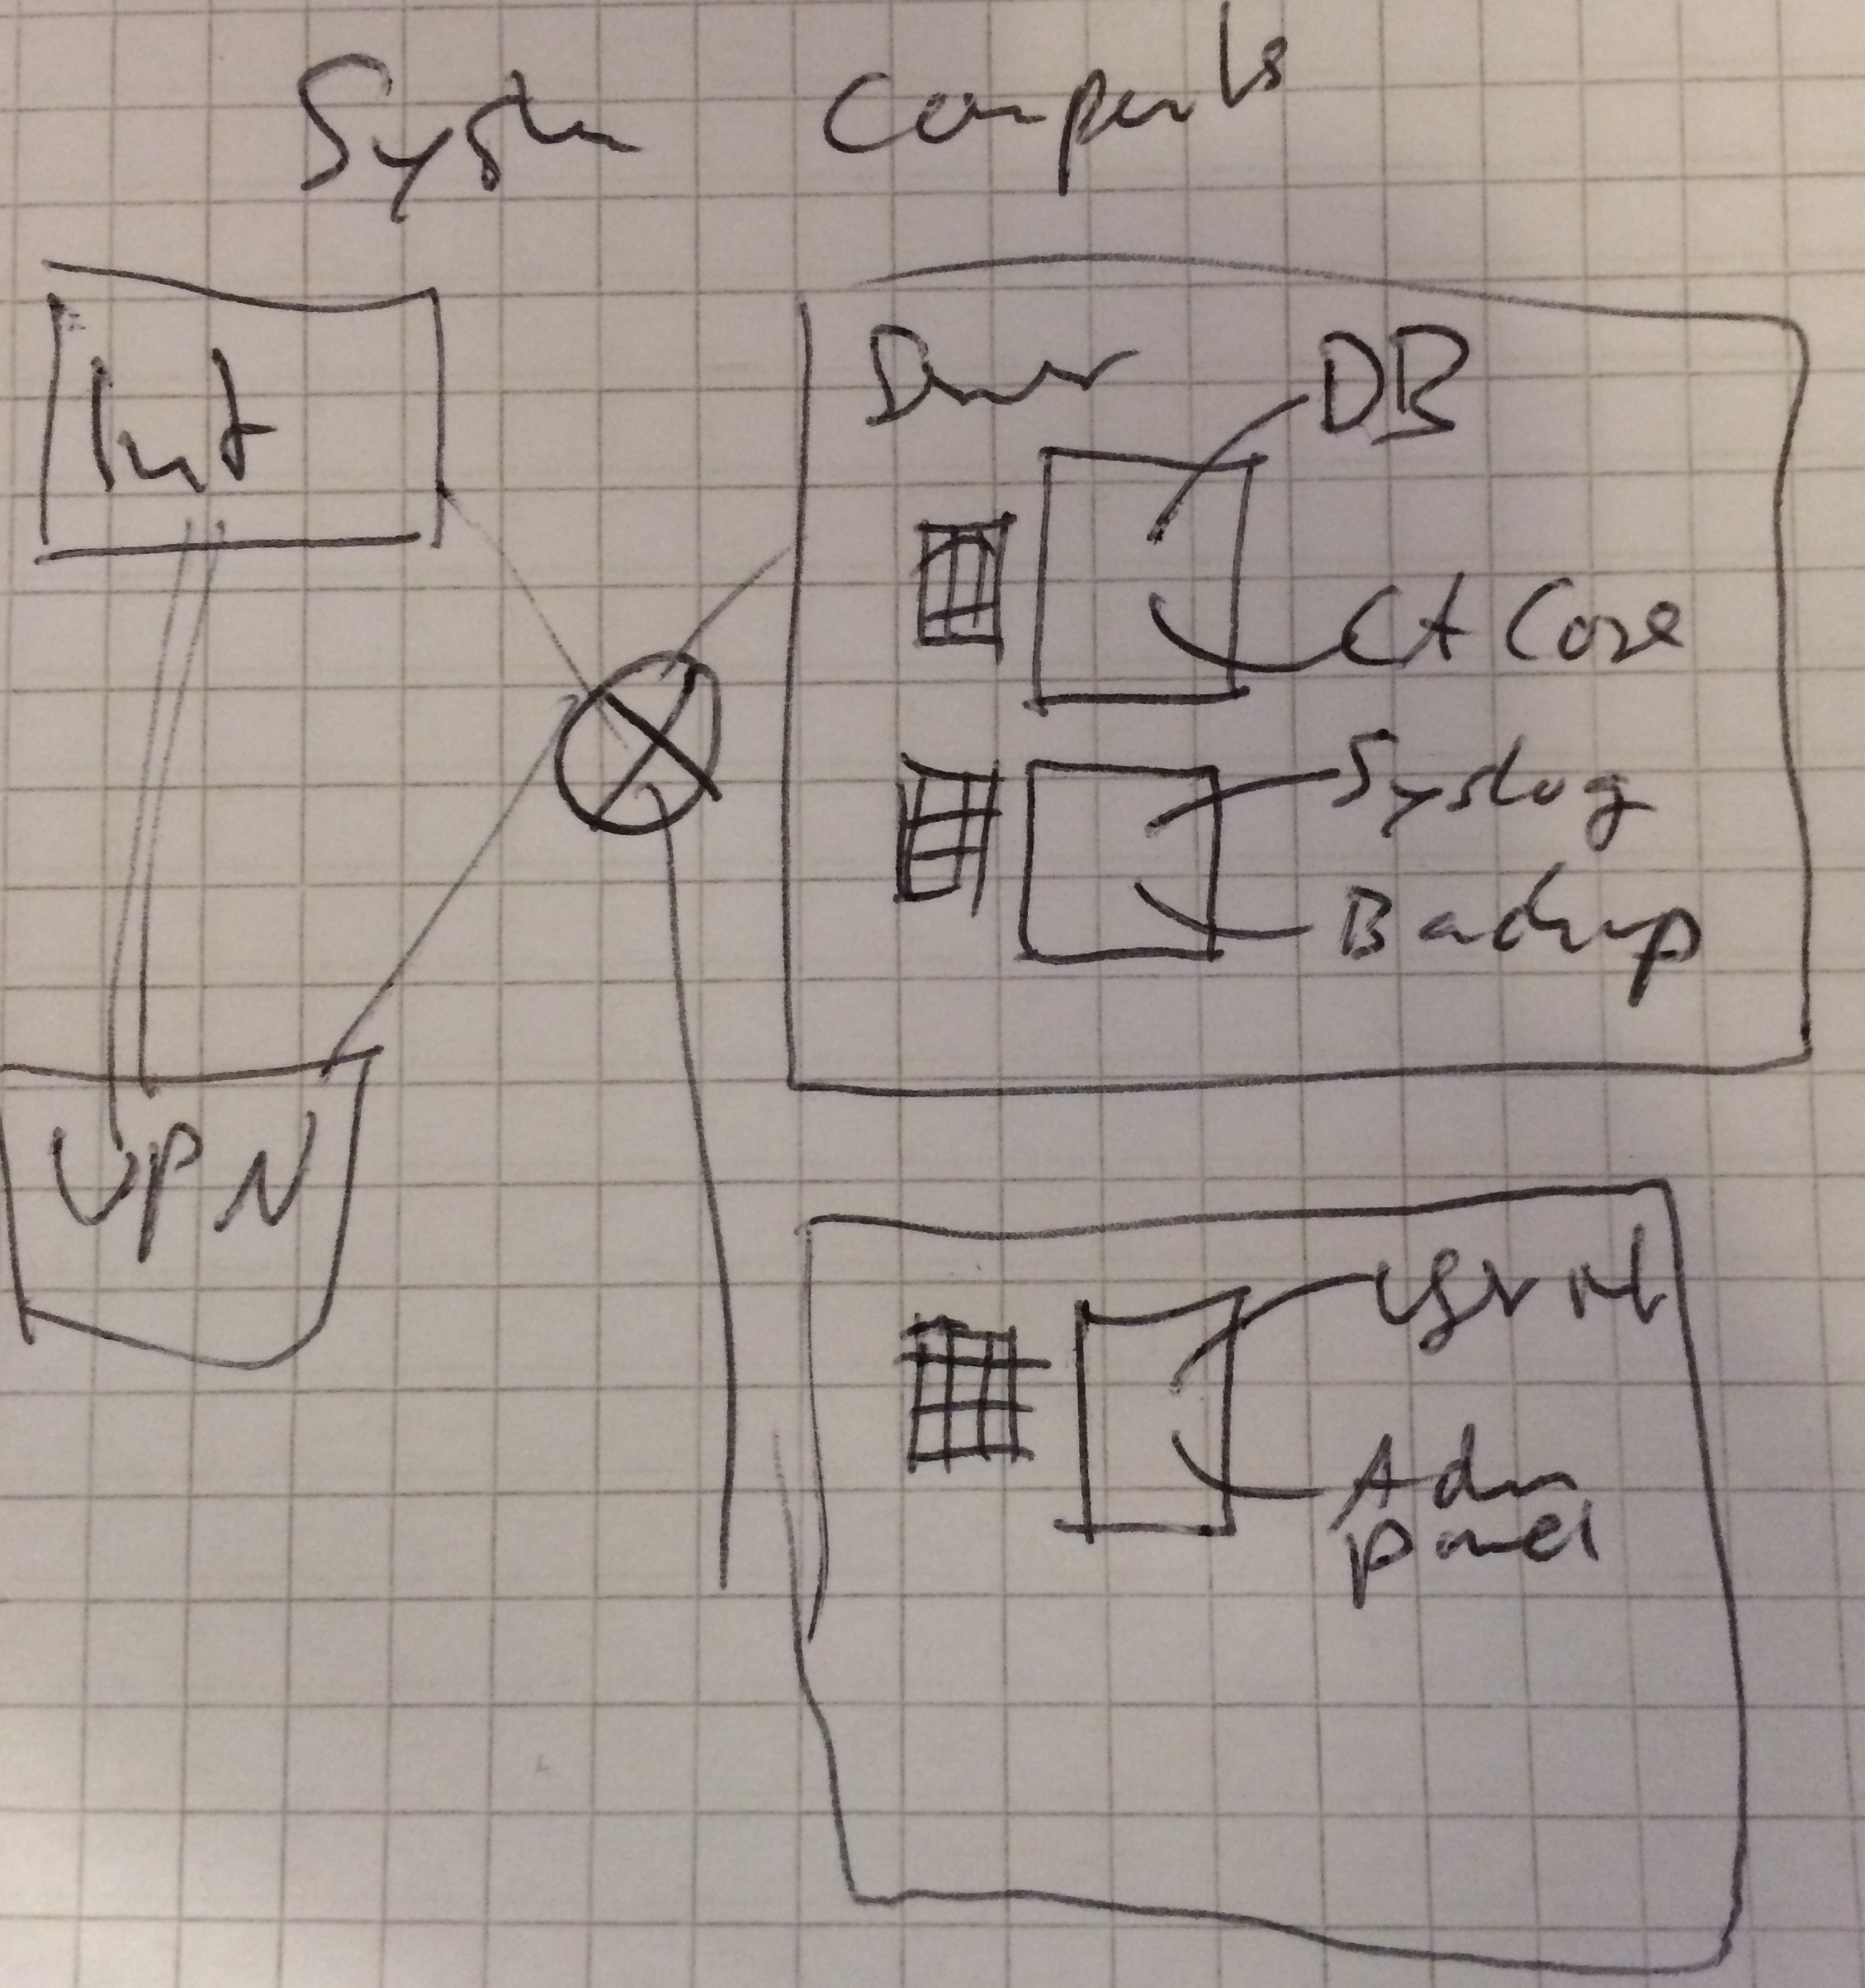
\includegraphics[width=0.6\textwidth]{images/systemcomponents.jpg}  
  \caption{Components of the proposed system.}
  \label{systemcomponents}
\end{figure}

\subsection{Platforms}
The components (as depicted in Figure \ref{systemcomponents}) are as follows:
\begin{description}
\item[Main Firewall] A software firewall based on Linux (IPCop) that divides the iMovies network into the parts DMZ, internal server network, office network and the internet. The firewall functions as a VPN endpoint for remote administrative access and restricts traffic between the subdivided networks according to a security policy described later.

\item[Web Server] A Linux machine running debian 7.0. It hosts the website for the user web interface and the administrative panel. The web server is located within the DMZ, a local iptables firewall allows only HTTPS connections to the outside and SSH connections to the firewall for administration, to the CA Core for secure RPC calls and to the backup server for secure backup and syslog.

\item[CA Core Server] A Linux machine running debian 7.0. It hosts the logic for issuing, verifying and revoking certificates as well as the legacy MyQSL database. The server is located within the internal server network, a local iptables firewall allows only SSH connections to the firewall for administration, to the web server for secure RPC calls and to the backup server for secure backup, syslog and key backup.

\item[Backup/Archive Server] AA Linux machine running debian 7.0. It hosts a syslog server, the logic for periodic backups and storage for encrypted key backup. The server is located within the internal server network, a local iptables firewall allows only SSH connections to the firewall for administration, to the web server and CA Core server for secure backup, syslog and key backup.
\end{description}

\subsection{Applications}

\begin{description}

\item[User Web Interface] Web application, developed in python running on nginx on the web server that allows the user to issue, verify and revoke certificates as well as view and alter user data. The website interacts with the CA Core via RPC calls.

\item[Administration Panel] Web application, developed in python running on nginx on the web server that allows the CA Administrator to review user changes and display information about the CAs status. The website interacts with the CA Core via RPC calls.

\item[Legacy DB] MySQL database with the legacy schema. Running on the CA Core server.

\item[CA Core] Application using the OpenSSL library that provides basic interfaces to create new key pairs, sign existing key pairs and revoke certificates. Running on the CA-Core server,  interacting with the web server via RPC calls and backing up private keys on the archive server via SSH.

\item[CA Core Storage] A database that is used by the CA Core to store certain data relevant to the CA Core application. Running on the CA Core server.

\item[Archive] Storage for encrypted public keys and certificates on the Backup/Archive server

\item[Backup] A script that collects via SSH and keeps multiple backups from the other servers (especially of all the configurations), running on the Backup/Archive server.

\item[Syslog] A Syslog server that receives logging data via SSH tunnel from the other servers, running on the Backup/Archive server.
\end{description}

\subsection{Data}

\begin{description}

\item[User Information] Basic information according to the schema of the legacy database. This includes the users username, his first and last name, his email address and a hash of his password. This information is stored in the legacy database.

\item[Key Pairs] Consist of a private key and the according public key that the CA Core generates on request. They are stored permanently in the archive and can be downloaded by the user. It is important, that the CA Core destroys his record of the private key as soon as possible.

\item[Certificates] A certificate that is signed by the CA Core. It is also stored in the archive and additionally also in the CA Storage (to allow certificates to be revoked).

\item[Certificate Revocation List] A list of certificates, that have been revoked by the CA Core. Stored on the CA Core server.

\item[Local Users] Credentials, that are used for system administration and communication between the components of the system. Individual to each system.

\item[Configuration Files] Configuration files define the configuration of a given system. They are in place at the system in question and backed up to the Backup/Archive server.

\item[Log Files] Log files generated by systems and applications. Stored on the Backup/Archive server.

\end{description}


\subsection{Interfaces}
\begin{description}

\item[Web Interface ]
Different for user and CA Administrator but in general it offers a way of authentication via credentials or certificate. Information flows from the outside through this interface via secure RPC calls into the CA Core and vice versa in which case the information gets displayed.

\item[Legacy DB Interface ]
Offers the functionality to ask for, alter and insert information to and from the database.

\item[CA Core Interface ]
Gets accessed via a RPC call to offer functionality to issue, revoke or verify certificates.

\item[Backup/Archive Interface ]
Implements syslog functionality to provide a syslog endpoint as well as storage for key and configuration backup.
\end{description}


\section{Implementation}
This section describes the implementation of our hardware and software with an emphasis on the security measures installed.
\begin{description}
\item[Main Firewall ] The Main Firewall is a software firewall running the IPCop Linux. It functions as a firewall as well as a router and divides the network into the sections DMZ, internal server network, office network (which is not implemented here), internet and VPN network. The routes to the known hardware of the iMovies infrastructure are statically assigned as well as the ARP tables to prevent poisoning. The firewall maintains a VPN using OpenVPN to allow remote access to the VPN network. Remote access to the firewall is possible via SSH out of the VPN network or via webinterface from address 10.10.10.33 from within the internal server network. \newline
The firewall implements several rules on how traffic is allowed to flow between those networks. By default all traffic is denied and silently dropped at the firewall. The following list shows the allowed exceptions: \newline
\begin{tabular}{p{2.5cm} c l p{4cm}}
Source & Protocol & Destination & Description\\
\cline{1-4}
Webserver & HTTPS (443) & Internet & Allow secure webtraffic from the webserver \\
\cline{1-4}
Internet & HTTPS (443) & Webserver & Allow secure webtraffic to the webserver\\
\cline{1-4}
10.10.10.33 & IPCop HTTPS (8023) & MainFirewall & Allow the use of the webinterface\\
\cline{1-4}
OpenVPN network & IPCop SSH (8022) & MainFirewall & Allow remote administrative access\\
\cline{1-4}
BackupServer & IPCop SSH (8022) & MainFirewall & Allow backup\\
\cline{1-4}
OpenVPN network & SSH (22) & Backupserver & Allow remote administrative access \\
\cline{1-4}
OpenVPN network & SSH (22) & CACore & Allow remote administrative access \\
\cline{1-4}
OpenVPN network & SSH (22) & Webserver & Allow remote administrative access \\
\cline{1-4}
Backupserver & SSH (22) & Webserver & Allow backup and tunneled syslog\\
\cline{1-4}
Webserver & SSH (22) & CACore & Allow tunneled RPC calls\\
\cline{1-4}
CACore & SSH (22) & Webserver & Allow tunneled RPC calls \\
\end{tabular}

\item[Servers in general ] We deploy three servers, the web server, the CA Core server and the Backup/Archive server. All servers are running debian in version 7.0. They have three users, root, an admin and an operational user. The operational user is not in the sudoers list and cannot get root access and should therefore be used to run the applications. We deactivated su and only allow sudo. Per default we deny all access via PAM (the Pluggable Authentication Modules). We ensure that the root user can only login locally and disable remote login. Failed login attempts get logged and automatically transmitted to the syslog server located on the Backup/Archive server. To prevent poisoning, we fix the ARP tables with the MAC addresses of all interacting systems. \newline
SSH is used for various interactions. We only allow the admin user and the operational user to have SSH access. With the help of sshguard we introduce a exponential time delay after three failed login attempts by implementing temporary rules to the local iptables. \newline
Each server has a local firewall based on iptables which blocks all connections by default. The exceptions are specific to the server and listed in their detailed implementing description.\newline
On the servers, the number of running processes is kept to a minimum, especially processes with network capabilities. With the help of the debian harden package, all unnecessary packages like telnet were removed. The services running on every system are sshd and rsyslogd. Some systems run additional services which are specified later. 

\item[Webserver ] The basic setup is as described in {\bfseries servers in general}. As the webserver needs additional functionality for running the websites and interacting with the CA Core, some more details have to be provided.\newline
The webservice used is nginx which was modified to only accept HTTPS request, meaning redirecting HTTP requests to HTTPS. Also there were measurements taken to minimize information leakage through server status and error pages. DESCRIBE HERE WHAT WAS DONE. ALSO DECRIBE WHAT COULD BE DONE AGAINST DDOS ETC.\newline
The two applications, the user web interface and the admin panel are developed in python. Both applications were written with  \texttt{Flask}, a microframework for web development. This open source framework provides all neccessary tools to build a simple and secure web application. For the encrypted interaction with the legacy database and the CA-Core we are using Pyro4, a distributed object middleware, which enables the web applications the communication with the CA-Core. The secrecy and integrity of these RPC calls are ensured by tunneling these calls via SSH to the CA Core server.\newline
To prevent cross-site request forgery (CSRF) attacks we are using the CRSF token provided by the flask framework and the user inputs are sanitized in flask automatically to render cross-side script (XSS) attacks impossible.\newline
In the case, that a adversary tries such attacks the two applications have a fine log system, that every access to a site with the given parameter is logged on the webserver. \newline
As all the servers, the webserver has a local iptables firewall which silently drops everything by default and implements the following exceptions:\newline
\begin{tabular}{p{2.5cm} c l p{4.5cm}}
Source & Protocol & Destination & Description\\
\cline{1-4}
Backupserver & SSH (22) & Webserver & Allow backup\\
\cline{1-4}
OpenVPN network & SSH (22) & Webserver & Allow remote administrative access \\
\cline{1-4}
Internet & HTTPS (443) & Webserver & Allow secure web traffic\\
\cline{1-4}
CACore & RPC (4444) & Webserver & Allow tunneled RPC call\\
\cline{1-4}
Webserver & HTTPS (443) & Internet & Allow secure web traffic\\
\cline{1-4}
Webserver & RPC (4444) &  CACore& Allow tunneled RPC call\\
\cline{1-4}
Webserver & syslog (10514) & Backupserver & Allow tunneled syslog\\
\cline{1-4}
CACore & SSH (22) & Webserver & Allow tunneled RPC call\\
\cline{1-4}
Webserver & SSH (22) & Backupserver & Allow tunneled syslog\\
\end{tabular}

\item[CA Core ] In addition to the basic setup described in {\bfseries servers in general}, the CA Core server houses the legacy MySQL database and the application that provides the functionality of issuing, verifying and revoking certificates. \newline
The MySQL database grants access to the table iMovies.users via the database user dbuser. This user only has limited rights, namely he can INSERT, SELECT and UPDATE only. There is no need for encrypting SQL traffic, since the database is on the same host as its consumer.\newline
The application who implements the certificate authority functionality works as follows DESCRIBE WHAT YOU IMPLEMENTED IN WHAT LANGUAGES, WHICH LIBRARIES WERE USED, HOW RPC IS IMPLEMENTED, WHAT WAS DONE IN TERMS OF SECURTY, DELETION OF PRIVATE KEY, HOW DOES THE PRIVATE KEY BACKUP WORK, MAYBE ALSO MENTION LOGGING.\newline
The interaction with the webserver happens via RPC calls over a SSH tunnel to ensure the security requirements. The same is true for the backing up of the private key, which gets moved to the Archive/Backup server through a SSH tunnel.\newline
The CA Core also implements a local, iptables based firewall which denies everything by default with these exceptions:\newline
\begin{tabular}{p{2.5cm} c l p{4.5cm}}
Source & Protocol & Destination & Description\\
\cline{1-4}
Backupserver & SSH (22) & CACore & Allow backup \\
\cline{1-4}
OpenVPN network & SSH (22) & CACore & Allow remote administrative access  \\
\cline{1-4}
Webserver & RPC (4444) & CACore & Allow tunneled RPC call \\
\cline{1-4}
CACore & RPC (4444) & Webserver & Allow tunneled RPC call \\
\cline{1-4}
CACore & SSH (22) & Backupserver & Allow key backup \\
\cline{1-4}
CAcore & syslog (10514) & Backupserver & Allow tunneled syslog\\
\cline{1-4}
Webserver & SSH (22) & CACore & Allow tunneled RPC call \\
\cline{1-4}
CACore & SSH (22) & Webserver & Allow tunneled RPC call \\
\end{tabular}


\item[Archive/Backup server ] The functionality this server implements in addition to the basic setup described in {\bfseries servers in general} is storage for the backed ups private keys, a script that backs up the configurations of the servers and a rsyslog server that collects the syslog data sent by the other machines and applications. Backup, syslog and key backup is done directly via SSH or via an SSH tunnel.\newline
The local iptables firewall that closes all ports by default implements the following exceptions:\newline
\begin{tabular}{p{2.5cm} c l p{4.5cm}}
Source & Protocol & Destination & Description\\
\cline{1-4}
CACore & SSH (22) & Backupserver & Allow key backup\\
\cline{1-4}
OpenVPN network & SSH (22) &  Backupserver & Allow remote administrative access\\
\cline{1-4}
Backupserver & SSH (22) & CACore & Allow backup\\
\cline{1-4}
Backupserver & SSH (22) & MainFirewall & Allow backup\\
\cline{1-4}
Backupserver & SSH (22) & Webserver & Allow backup\\
\cline{1-4}
Webserver & syslog (10514) & Backupserver & Allow tunneled syslog\\
\cline{1-4}
CAcore & syslog (10514) & Backupserver & Allow tunneled syslog\\
\end{tabular}
\end{description}


\section{Operation}
During operation of the system several actions can be performed to keep the system secure and detect misuse or an attack early on. \newline
\begin{description}
\item[Update ] Perform regular updates of all system software to avoid security holes.
\item[Logging ] Evaluate the logs and look for anomalies unintended patterns.
\item[Audit ] Make sure that the information in the logs can be linked to a specific user and action for accountability.
\item[Backup ] Check that the backups work and also check if playing back a backed up configuration would work.
\item[Detection ] Try to detect misuse with monitoring programs. Like monitoring overall network traffic which should be fairly low under normal usage or run intrusion detection systems. The installed libraries harden-nids for network intrusion detection and harden-surveillance for network surveillance from the harden package can help with that task.
\end{description}


\section{System documentation}
This section is in some sense a summary of the above with some additional information about the systems like usernames, passwords, IP addresses, virtual network names etc. Use this section for administrative purposes of the system.\newline

\subsection{Network diagram}

\begin{figure}[H]
  \centering
    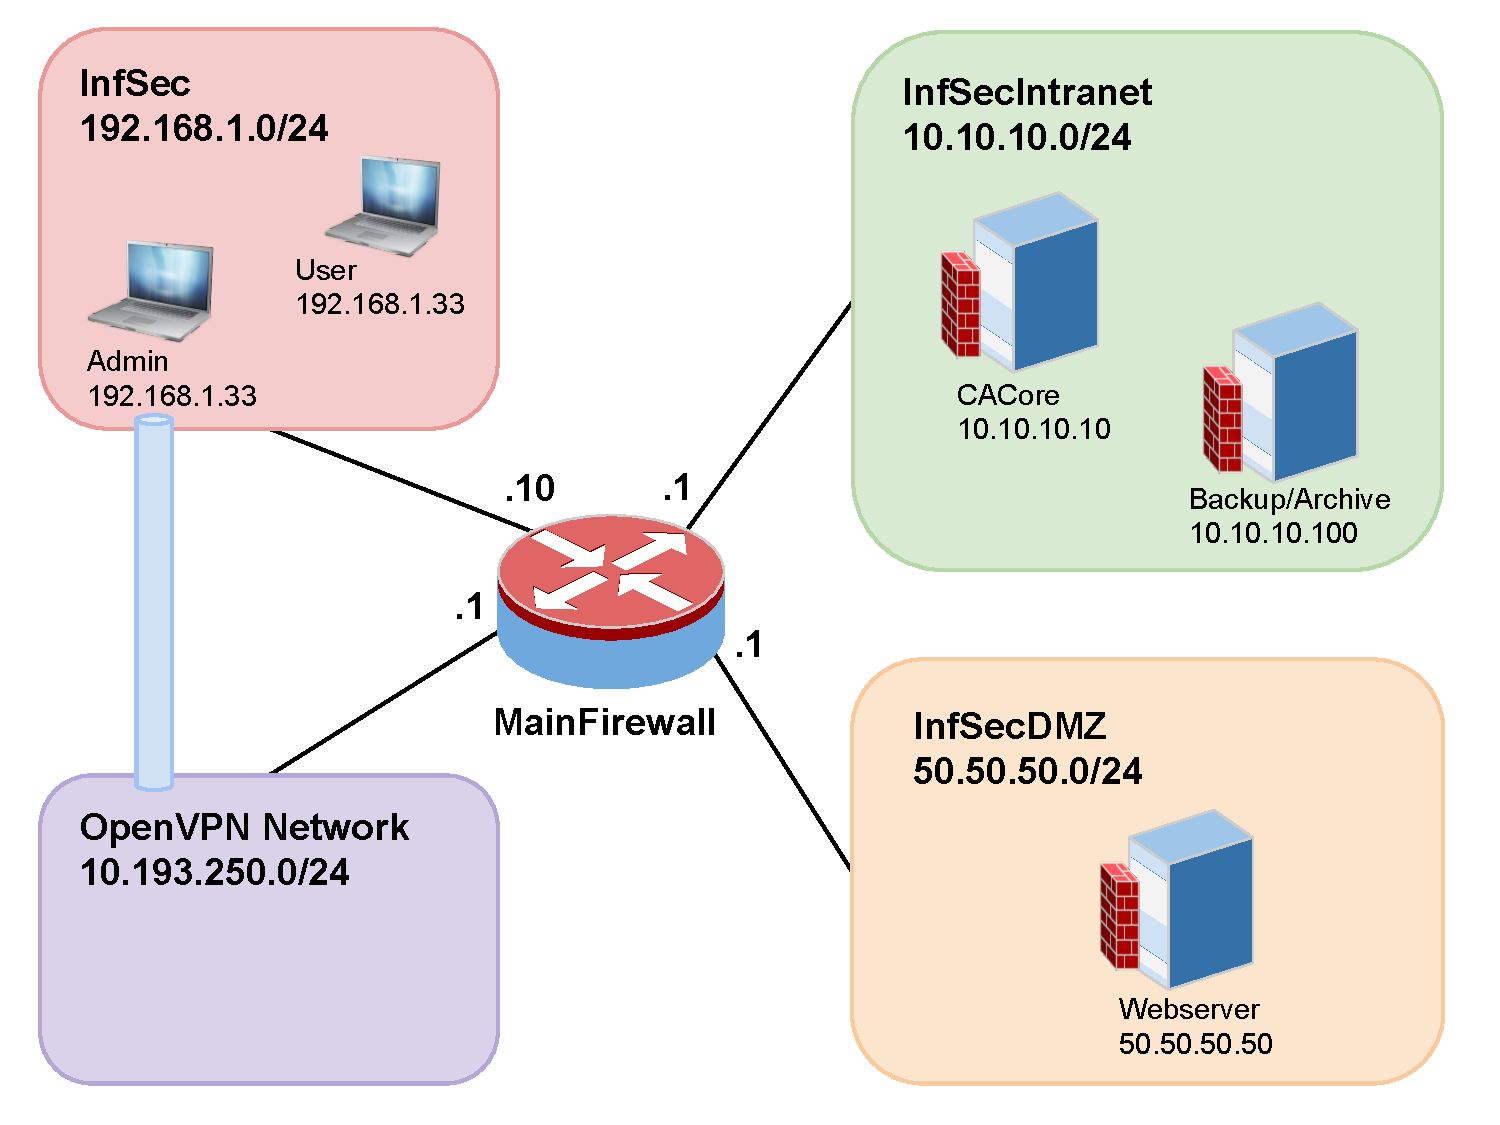
\includegraphics[width=0.9\textwidth]{images/sysseclab_net_diagram.pdf}  
  \caption{Network Diagram}
  \label{netdiag}
\end{figure}

\subsection{Machines}
All servers are equipped with at least one NIC corresponding to the network they are in as shown in Figure \ref{netdiag} and a NAT NIC that can be used for internet access (git, apt-get, etc.).
\subsubsection{MainFirewall}
\subsubsection*{Accounts \& Passwords}
\begin{multicols}{2}
\begin{description}
\item[admin:] wT7nDB7A7d7V
\item[root:] 5hmAMWxN6uVa
\end{description}
\end{multicols}
\subsubsection*{Installed software}
IPCop
\subsubsection*{User for ssh access}
Accesable only on 10.10.10.1 with port 8022 from 10.10.10.33 (user in InfSecIntranet) or from OpenVPN-Network.\newline
ssh -p 8022 admin@10.10.10.1
\subsubsection*{Additional information}
There is a webinterface on https://10.10.10.1:8023. Only accessable from 10.10.10.33 (user in InfSecIntranet).

\subsubsection{Webserver}
\subsubsection*{Accounts \& Passwords}
\begin{multicols}{2}
\begin{description}
\item[serveruser:] 3FaVLt9RNxLu
\item[root:] cLepMVRq8wDQ
\item[operuser:] KLs3PbjoXu9m
\end{description}
\end{multicols}
operuser cannot use sudo/su and should therefore be used to run the application.
\subsubsection*{Installed software}
Debian, iptables, nginx, python, flask, openSSL, openSSH
\subsubsection*{Running services (lsof -i)}
sshd, nginx
\subsubsection*{User for ssh access}
ssh \{operuser, serveruser\}@50.50.50.50
\subsubsection*{additional information}
SSL signing key for HTTPS: 9klTRxBQcAnM

\subsubsection{CoreCA}
\subsubsection*{Accounts \& Passwords}
\begin{multicols}{2}
\begin{description}
\item[causer:] 9BxkXM5fLLL8
\item[root:] 8kSeddphG6Ac
\item[operuser:] PrCgs5TLqW4f
\end{description}
\end{multicols}
operuser cannot use sudo/su and should therefore be used to run the application.
\subsubsection*{Installed software}
Debian, iptables, python, mySQL, openSSL, openSSH
\subsubsection*{Running services (lsof -i)}
sshd, mysql (only localhost)
\subsubsection*{User for ssh access}
ssh \{operuser, causer\}@10.10.10.10
\subsubsection*{additional information}
MySQL root: Cm7NsWBhf52C\newline
MySQL dbuser: Q8mxLsBwTLJi\newline
dbuser is only allowed to INSERT, SELECT, UPDATE the table user.iMovies, thus should be used for connecting to the database.

\subsubsection{Backup/Archive Server}
\subsubsection*{Accounts \& Passwords}
\begin{multicols}{2}
\begin{description}
\item[archiveuser:] 4uMtrPMLxShw
\item[root:] gaBWUt5EH8vU
\item[operuser:] QT5wbxjCN8gG
\end{description}
\end{multicols}
operuser cannot use sudo/su and should therefore be used to run the application.
\subsubsection*{Installed software}
Debian, iptables, syslog, openSSH
\subsubsection*{Running services (lsof -i)}
sshd
\subsubsection*{User for ssh access}
ssh \{operuser, archiveuser\}@10.10.10.100

\subsubsection{User}
\subsubsection*{Accounts \& Passwords}
\begin{description}
\item[alice:] alice
\end{description}
\subsubsection*{additional information}
When running in netwok InfSec, VPN is possible (VPN start script on Desktop):\newline
\begin{description}
\item[PKCS12 PW:] StgmE58sadQu
\end{description}
When running in netwok InfSecIntranet, firewall web access on https://10.10.10.1:8023


\subsection{Firewall rules}
\subsubsection{MainFirewall}
All connections are closed by default. The following list shows the allowed exceptions:\newline

\begin{tabular}{l c l}
Source & Protocol & Destination \\
\cline{1-3}
Webserver & HTTPS (443) & InfSec \\
\cline{1-3}
InfSec & HTTPS (443) & Webserver \\
\cline{1-3}
10.10.10.33 & IPCop HTTPS (8023) & MainFirewall\\
\cline{1-3}
OpenVPN network & IPCop SSH (8022) & MainFirewall \\
\cline{1-3}
10.10.10.33 & IPCop SSH (8022) & MainFirewall \\
\cline{1-3}
BackupServer & IPCop SSH (8022) & MainFirewall \\
\cline{1-3}
OpenVPN network & SSH (22) & Backupserver \\
\cline{1-3}
OpenVPN network & SSH (22) & CACore \\
\cline{1-3}
OpenVPN network & SSH (22) & Webserver \\
\cline{1-3}
Webserver & RPC (4444) & CACore \\
\cline{1-3}
CACore & RPC (4444) & Webserver \\
\cline{1-3}
Backupserver & SSH (22) & Webserver \\
\cline{1-3}
Webserver & SSH (22) & CACore \\
\cline{1-3}
CACore & SSH (22) & Webserver \\
\cline{1-3}
Webserver & syslog (10514) & Backupserver \\
\end{tabular}

\subsubsection{Webserver}
All connections are closed by default. The following list shows the allowed exceptions:\newline


\begin{tabular}{c c c}
Source & Protocol & Destination \\
\cline{1-3}
Backupserver & SSH (22) & Webserver \\
\cline{1-3}
OpenVPN network & SSH (22) & Webserver \\
\cline{1-3}
InfSec & HTTPS (443) & Webserver \\
\cline{1-3}
CACore & RPC (4444) & Webserver \\
\cline{1-3}
Webserver & HTTPS (443) &  \\
\cline{1-3}
Webserver & RPC (4444) &  \\
\cline{1-3}
Webserver & syslog (10514) & Backupserver \\
\cline{1-3}
CACore & SSH (22) & Webserver \\
\cline{1-3}
Webserver & SSH (22) &  \\
\end{tabular}

\subsubsection{CoreCA}
All connections are closed by default. The following list shows the allowed exceptions:\newline


\begin{tabular}{c c c}
Source & Protocol & Destination \\
\cline{1-3}
Backupserver & SSH (22) & CACore \\
\cline{1-3}
OpenVPN network & SSH (22) & CACore \\
\cline{1-3}
Webserver & RPC (4444) & CACore \\
\cline{1-3}
CACore & RPC (4444) & Webserver \\
\cline{1-3}
CACore & SSH (22) & Backupserver \\
\cline{1-3}
CAcore & syslog (10514) & Backupserver \\
\cline{1-3}
Webserver & SSH (22) & CACore \\
\cline{1-3}
CACore & SSH (22) & Webserver \\
\end{tabular}

\subsubsection{Backup/Archive Server}
All connections are closed by default. The following list shows the allowed exceptions:\newline


\begin{tabular}{l c l}
Source & Protocol & Destination \\
\cline{1-3}
CACore & SSH (22) & Backupserver \\
\cline{1-3}
OpenVPN network & SSH (22) &  Backupserver\\
\cline{1-3}
Backupserver & SSH (22) & CACore \\
\cline{1-3}
Backupserver & SSH (22) & MainFirewall \\
\cline{1-3}
Backupserver & SSH (22) & Webserver \\
\cline{1-3}
Webserver & syslog (10514) & Backupserver \\
\cline{1-3}
CAcore & syslog (10514) & Backupserver \\
\end{tabular}



\section{Backdoors}

Describe the implemented backdoors. {\bfseries Do not add
    this section to the version of your report that is handed over to
    the team that reviews your system!}



\chapter{Risk Analysis and Security Measures}

\section{Information Assets}

Describe the relevant assets and their required security
  properties. For example, data objects, access restrictions,
  configurations, etc.

\section{Threat Sources}

Name and describe potential threat sources.

\section{Risks and Countermeasures}

List all potential threats and the
  corresponding countermeasures. Estimate the risk based on 
  the information about the threat, the threat sources and the 
  corresponding countermeasure. For this purpose, use the following three
  tables.

%\subsection{Tools}

\begin{center}
\begin{tabular}{|l|l|}
\hline
\multicolumn{2}{|c|}{\bf Impact} \\
\hline
Impact & Description \\
\hline
\hline
High   & \hspace*{20pt}\ldots \\
\hline
Medium & \hspace*{20pt}\ldots \\
\hline
Low   & \hspace*{20pt}\ldots \\
\hline
\end{tabular}
%
%\vspace{5mm}
%
%\noindent \hspace*{10pt}
\begin{tabular}{|l|l|}
\hline
\multicolumn{2}{|c|}{\bf Likelihood} \\
\hline
Likelihood & Description \\
\hline
\hline
High   & \hspace*{20pt}\ldots \\
\hline
Medium & \hspace*{20pt}\ldots \\
\hline
Low   & \hspace*{20pt}\ldots \\
\hline
\end{tabular}
\end{center}

\vspace{5mm}

\begin{center}
\begin{tabular}{|l|c|c|c|}
\hline
\multicolumn{4}{|c|}{{\bf Risk Level}} \\
\hline
{{\bf Likelihood}} & \multicolumn{3}{c|}{{\bf Impact}} \\ %\cline{2-4}
     & Low & Medium & High \\  \hline
 High & Low & Medium & High  \\
\hline
 Medium & Low & Medium & Medium \\
\hline
 Low & Low & Low & Low \\
\hline
\end{tabular}
\end{center}

\subsection{{\it Evaluation Asset X}}

Evaluate the likelihood, impact and the resulting risk,  after implementation of the corresponding countermeasures.

\begin{footnotesize}
\begin{prettytablex}{lXp{6.5cm}lll}
No. & Threat & Implemented/planned countermeasure(s) & L & I & Risk \\
\hline
1 & ... & ... & {\it Low} & {\it Low} & {\it Low} \\
\hline
2 & ... & ...& {\it Medium} & {\it High} & {\it Medium} \\
\hline
\end{prettytablex}
\end{footnotesize}



\subsection{{\it Evaluation Asset y}}

\begin{footnotesize}
\begin{prettytablex}{lXp{6.5cm}lll}
No. & Threat & Implemented/planned countermeasure(s) & L & I & Risk \\
\hline
1 & ... & ... & {\it Low} & {\it Low} & {\it Low} \\
\hline
2 & ... & ...& {\it Medium} & {\it High} & {\it Medium} \\
\hline
\end{prettytablex}
\end{footnotesize}

\subsection{Detailed Description of Selected Countermeasures}

Optionally explain the details of the countermeasures mentioned above.



\subsection{Risk Acceptance}

List all medium and high risks, according to the evaluation above. For each risk, propose additional countermeasures that could be implemented to further reduce the risks.

\begin{footnotesize}
\begin{prettytablex}{p{2cm}X}
No. of threat & Proposed countermeasure including expected impact  \\
\hline
... & ... \\
\hline
... & ... \\
\hline
\end{prettytablex}
\end{footnotesize}

\end{document}

%%% Local Variables: 
%%% mode: latex
%%% TeX-master: "../../book"
%%% End: 
